\lab{Algorithm}{Line Sweep and Voronoi Diagrams}{Line Sweep}
\label{lab:Alg_Linesweep}

\objective{Learn about and implement a basic line sweep algorithm and Introduce Voronoid Diagrams and Delaunay Triangulations and discuss their applications}

\section*{General Line Sweep Algorithms}

Line sweep algorithms are a significant group of algorithms with a variety of applications. 
In the strictest sense, line sweep algorithms typically use a priority queue and binary tree to lower the temporal complexity associated with certain tasks. 
Some notable examples include Fortune's Algorithm for calculating Voronoi diagrams and Andrew's Algorithm for computing the convex hull of a set of points. 
In this lab, we will explore a basic line sweep algorithm that allows efficient computation of the Closest Pair problem.  
Given a set of points, find the distance between the closest pair of points.

\section*{Na\"ive Implementation}

The obvious way of doing this is to simply compute the distance between each point and each of the other points.
Roughly speaking, this requires some constant multiple of $n^2$ computations where $n$ is the number of points.
This can be coded as follows:
\begin{lstlisting}
def reallybadmindist(X):
    r = ((X[0]-X[1])**2).sum()**.5
    for i in range(len(X)):
        for j in range(len(X)):
            if i != j:
                r = min(r,((X[i]-X[j])**2).sum()**.5)
    return r
\end{lstlisting}
Since distance is symmetrical, we can compare each point with the points that follow it in the list we are given (which will reduce
the total number of distances to be computed).
This is a slightly better implementation:
\begin{lstlisting}
def multidist(p0,p1):
    l=len(p0)
    return sum([(p0[i]-p1[i])**2 for i in range(l)])**.5
def badmindist(X):
    l=len(X)
    r=multidist(X[0],X[1])
    for i in xrange(l):
        for j in xrange(i+1,l):
            d=multidist(X[i],X[j])
            if d<r:
                r=d
    return r
\end{lstlisting}

Since, on average, we iterate through about half of the list for each point added, this algorithm will have complexity $O(n^2)$ (we are only scaling by a constant factor).  
It is faster than the truly na\"ive method, but essentially just as inefficient.
For very small numbers of points, this algorithm works, but it quickly becomes inefficient as we increase the number of points processed.  
What we would like to do is go from $O(n^2)$ to something better.  
To do this, we have to think about the problem differently.
This can be done by using one of the key techniques of computational geometry-a line sweep algorithm.

\section*{A Simplified Line Sweep Algorithm}

The concept behind a line sweep algorithm is breaking a global problem into a sequence of smaller problems that can be solved locally.
We sweep the domain space with a line.
This line divides the domain space into an explored region and an unexplored region.
As the line sweeps, events occur, be it whether the line encounters a point in the data set
or some other type of event.  
We compute the solution at the very beginning of the line sweep and as new events happen, we compute the change that these events have on our current solution.
We only need to consider the events in the explored region or on the sweep line as they are the only events that affect the current solution.  
Sweep line algorithms typically exhibit a temporal complexity of $O(n \log n)$, which is far better than $O(n^2)$.

Line sweep algorithms are good for doing all sorts of proximity based computations.
In the example above, we took advantage of the fact that distance was symmetric ($d(a,b)=d(b,a)$).
In a line sweep version of this algorithm, we also take advantage of the fact that any points further than the current smallest minimum distance along a given axis do not need to be considered.
This is really just an application of the triangle inequality.
The secret to the line sweep solution for the closest pair problem is to actually have two sweep lines with a small distance between them.
As we process the points in our list, we can decrease the distance between the lines so that we only process points that could possibly give a smaller distance than the smallest distance we have already encountered.
By only processing the points between our two sweep lines, we avoid processing many points needlessly.

For a general line sweep algorithm, it is common to use a priority queue to order the items that need to be processed.
A good priority queue can be found in the library \li{Queue} that is included in Python. 
In this case all we need to do is sort the points by $X$ value.
This means it will be easier to make a sorted copy of the array using Numpy's built in functions.
Something like \li{X=Y.take(Y[:,0].argsort(),axis=0)} or \li{Y[Y[:,0].argsort()]} will do this for you. 

We track the points in the area between the two sweep lines with a list.
Each time we advance the sweep lines, we update this list so it always contains the points between the sweep lines (adding or removing points where necessary).
A point stays in the list if its distance from the leading sweep line is less than the current minimum distance.
Conceptually, this is how we place the second sweep line.

Assuming we have already ordered all our points by $x$ coordinate, we can perform the line sweep algorithm as follows:

\vspace{5mm}
\begin{compactenum}[1.]
\item 
Process the first two points and add them to the active list.
Set current minimum distance to the distance between these two points.
\item 
Get the next point in the priority queue.
\item 
Update the active list so that it contains only the points between the two sweep lines.
\item 
Compute the distance between the current point and all the points in the active list.
\item 
Compare the smallest distance found with the current minimum distance. 
Change the current minimum distance if needed.
\item 
Repeat steps 2 to 5 for all remaining points in the priority queue
\end{compactenum}
\vspace{5mm}

When the algorithm ends, the current minimum distance will be the distance between the closest pair of points.

This algorithm can be illustrated as follows:
\begin{figure}[H]
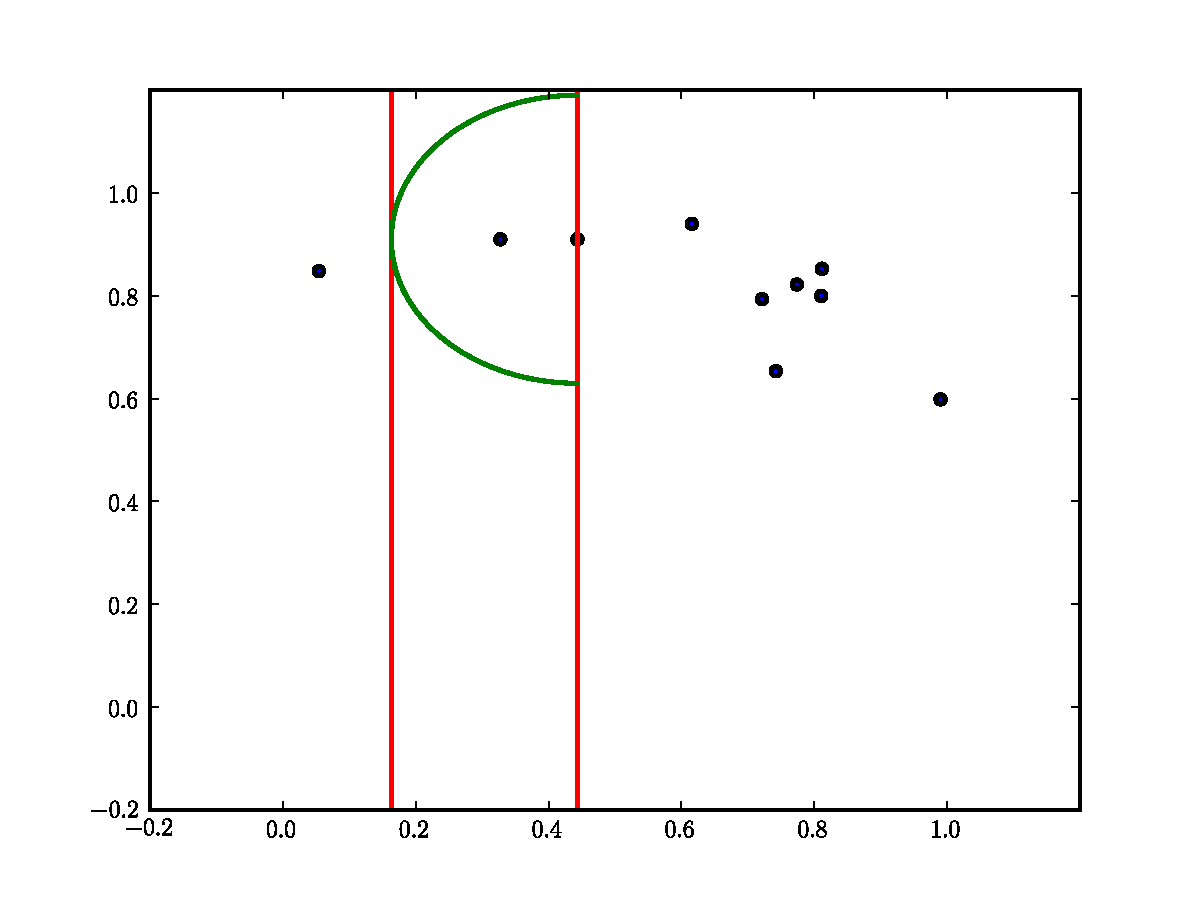
\includegraphics[width = .8\textwidth]{simple0.pdf}
\caption{After processing the first two points, we process the third point and change the current minimum distance accordingly.}
\end{figure}

\begin{figure}[H]
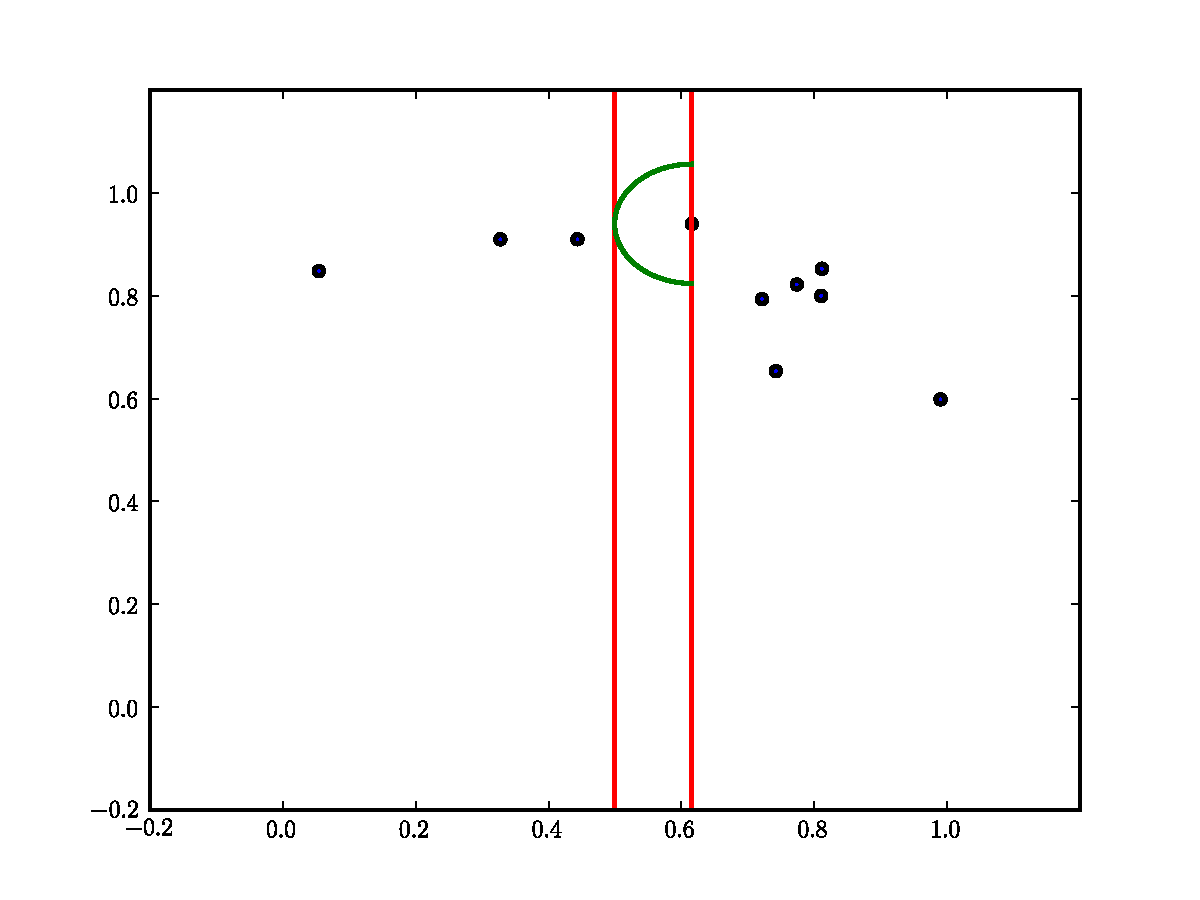
\includegraphics[width = .8\textwidth]{simple1.pdf}
\caption{This change in the minimum thus far is reflected in how we form the actives list for the next point we process. 
We remove the points from the top of the queue that are too far away in the $x$ direction to have a distance less than the current minimum. 
We then process anything that is left.}
\end{figure}

\begin{figure}[H]
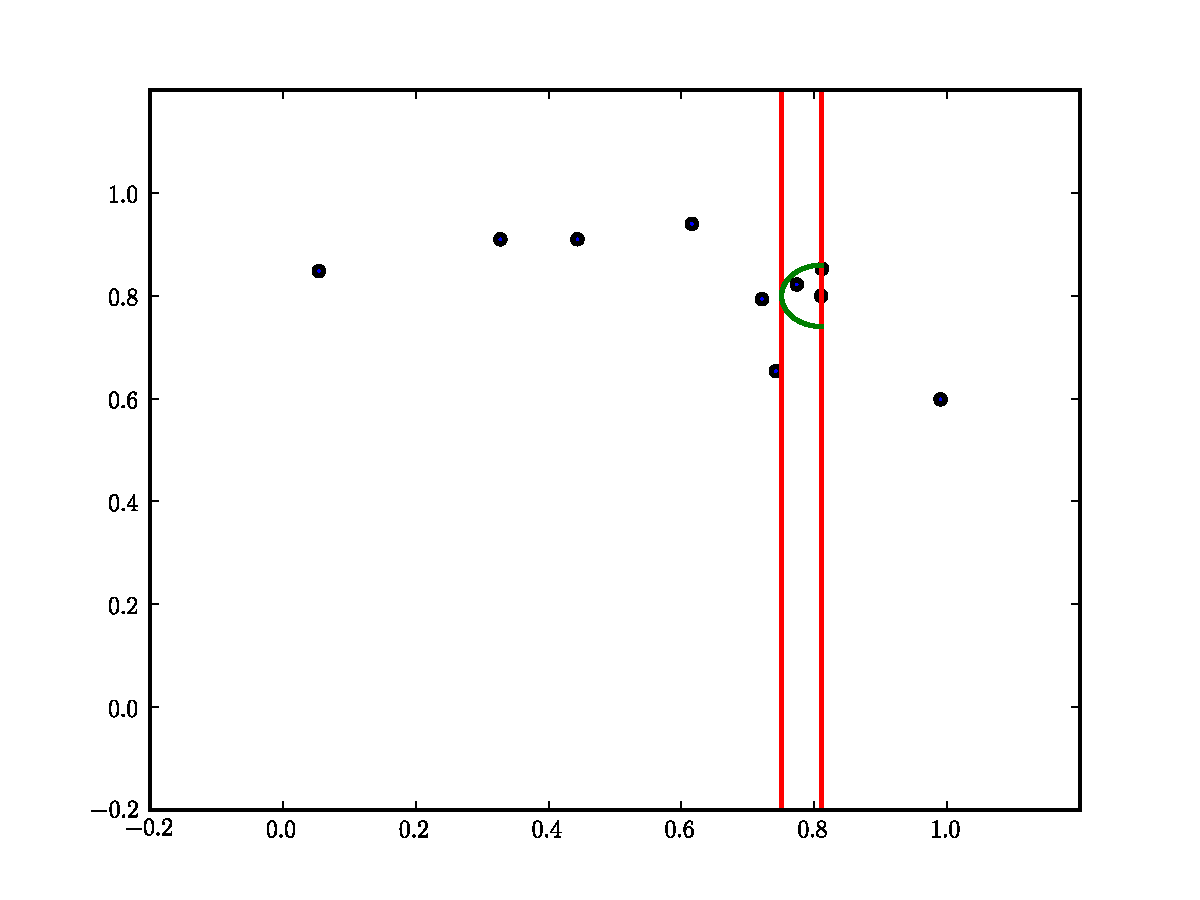
\includegraphics[width = .8\textwidth]{simple5.pdf}
\caption{A few points further in we actually hit the minimum distance.}
\end{figure}

\begin{figure}[H]
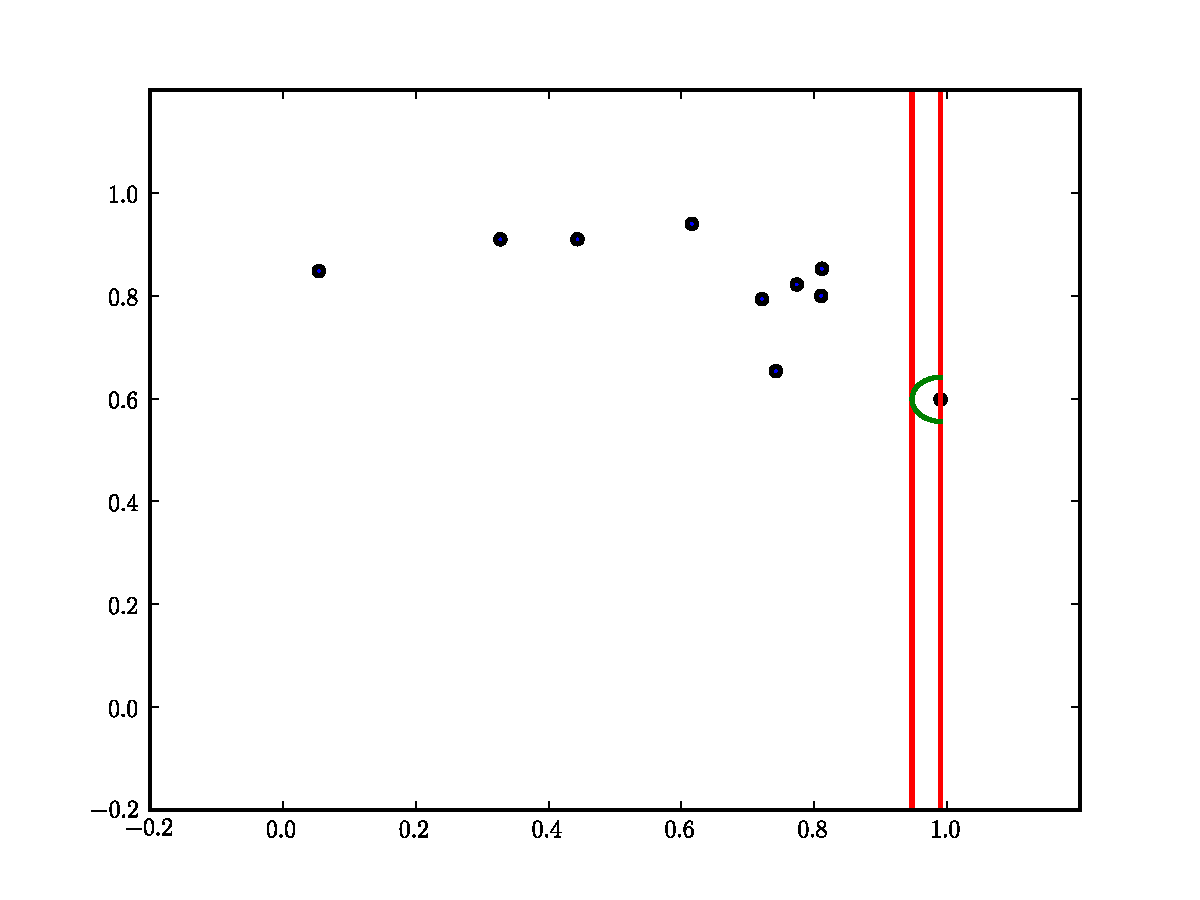
\includegraphics[width = .8\textwidth]{simple7.pdf}
\caption{After iterating over all the points in the set, we have the final minimum distance desired.}
\end{figure}

\begin{problem}
Write a Python function that implements the above algorithm.
Have your code accept a metric function as a parameter.
This metric function should take a point and an array of points as arguments and return an array of distances from the point to each of the points in the array. 
Test your function's speed. 
How does it scale as you increase the number of points? 
How does it scale as you increase the number of dimensions?
\end{problem}

\section*{A Line Sweep Algorithm}

You may have noticed that we are not exploiting all the symmetry of the problem in the previous algorithm. 
It would likely speed things up if we could also slice away the points that have $y$ values that could not possibly yield the minimum distance. 
The simplest way to do this in this case is to take advantage of some algebraic symmetry.
As we compute the distance between two points, we have to calculate the difference between each of the coordinates of the points in question. 
If at any time the difference has an absolute value greater than the minimum distance we have encountered thus far, we know we don't need to finish processing the point.
This is, theoretically, like slicing along the other axes in order to further reduce the ``active'' list of points.
A similar result could be obtained by using a list, binary tree, or some other data structure to keep the list of active points sorted by $y$ value, but in this case the insertion and deletion operations involved are more costly.

This algorithm can be illustrated as follows:

Note: in this case we sweep along the $x$ axis from right to left.

\begin{figure}[H]
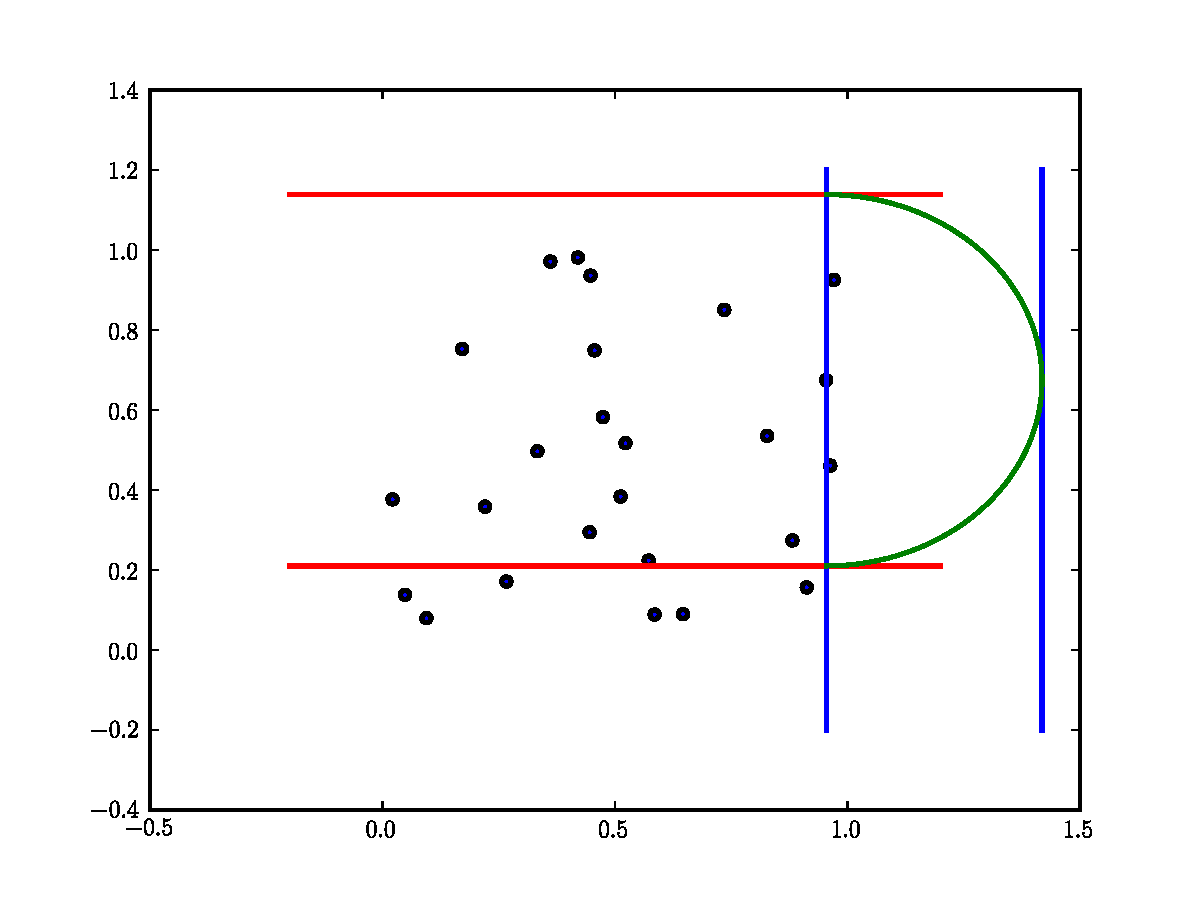
\includegraphics[width = .8\textwidth]{sweep0.pdf}
\caption{In processing the first point, we find find that we must reduce the radius.
Notice that we only need to consider the points that lie in the box formed by the red an blue lines.}
\end{figure}

\begin{figure}[H]
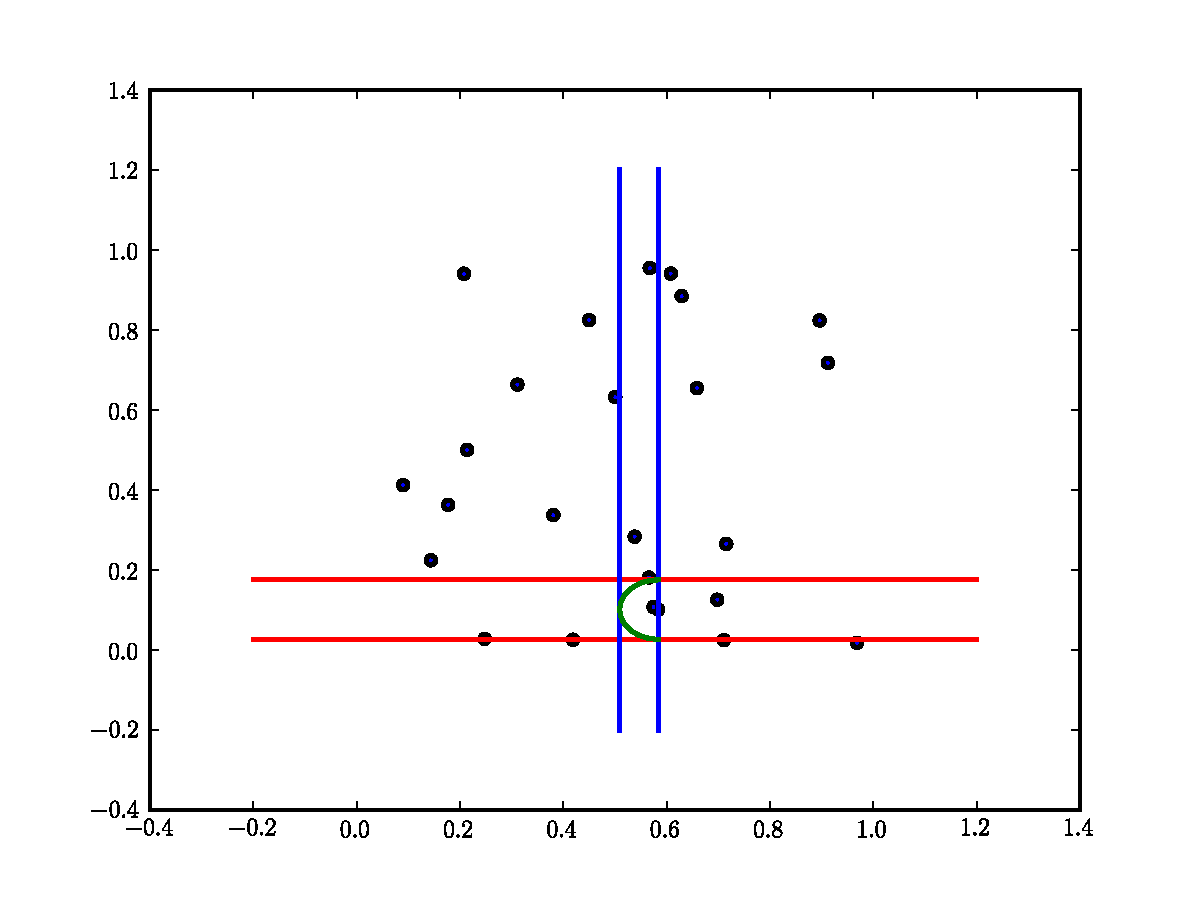
\includegraphics[width = .8\textwidth]{sweep13.pdf}
\caption{This is where we actually hit the minimum distance.}
\end{figure}

\begin{figure}[H]
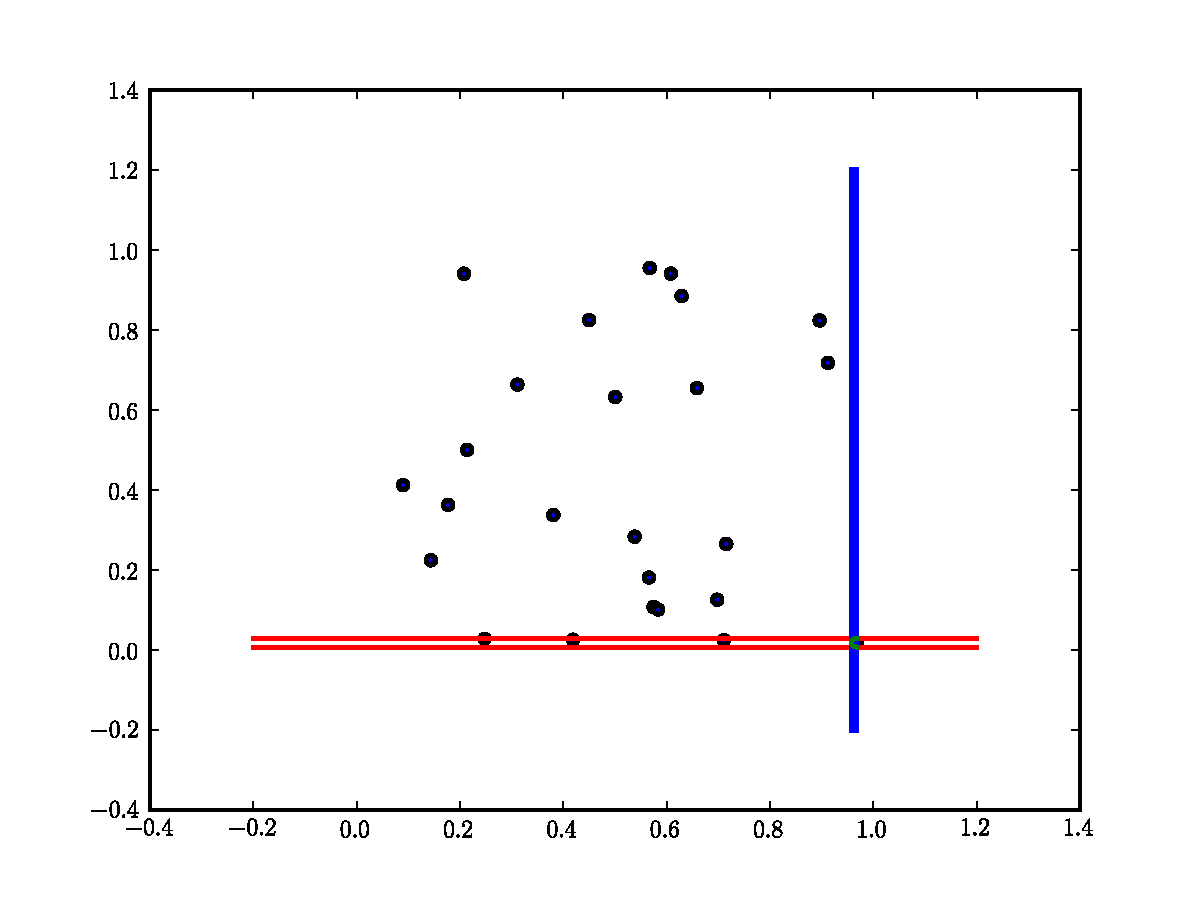
\includegraphics[width = .8\textwidth]{sweep22.pdf}
\caption{After processing through all the points, we are guaranteed to have hit the minimum distance already, so our minimum distance thus far is our final return value.}
\end{figure}


\begin{problem}
Implement the algorithm above in Python. 
Time it against the naive implementation at the beginning of this lab and against the simplified version you coded above.
The new version should be faster, but speed depends heavily on how you have implemented it, so you may have some optimization left to do.
Time how long it takes your new function to process ten million points in two dimensions. 
Using benchmarks from the first implementation we gave you, estimate how long (in years) it would take that function to process that many points.
How many times faster is the good implementation?
\end{problem}

Since this version of the algorithm depends so heavily on array lookups, it will be much faster if it is implemented in Cython.

\section*{Voronoi Diagrams}

In this section we will discuss some applications of Voronoi Diagrams.
They are an application of the line sweep algorithm in that they can be computed using a line sweep algorithm called Fortune's Algorithm.
In the abstract sense, a Voronoi diagram is a partition of a plane into regions that lie closest to different points.
The easiest way to understand this is to look at some examples.
Figure \ref{voronoi_ex_1} is a voronoi diagram generated from 100 random points with $x$ and $y$ values between 0 and 1.
Notice how each point has a small  cell around it that is made up of the points that lie closest to it.

\begin{figure}
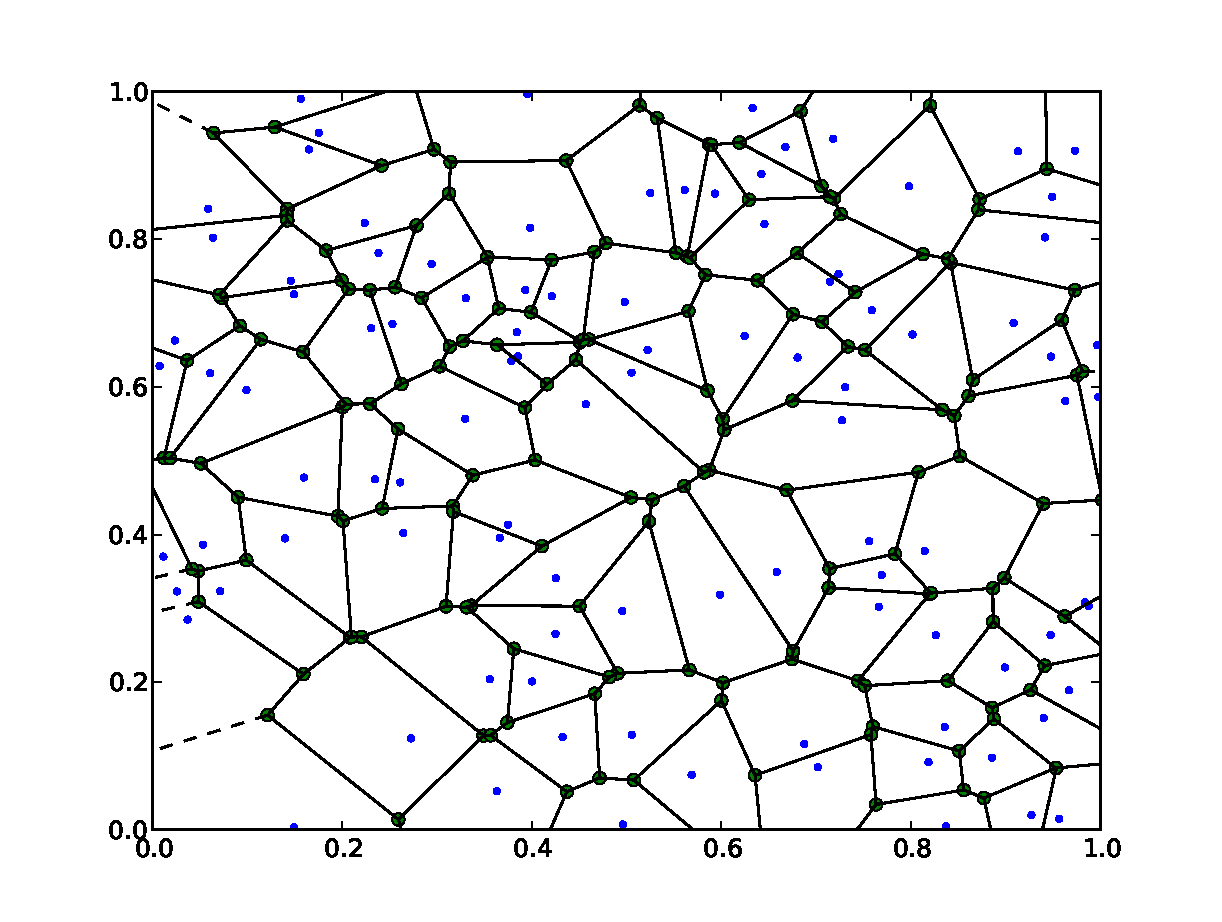
\includegraphics[width=\textwidth]{voronoi_example_1.pdf}
\caption{A Voronoi diagram of the square $[0,1]\times [0,1]$ for 100 randomly generated points.}
\label{voronoi_ex_1}
\end{figure}

One possible way to compute this sort of diagram would be by brute force, for example:
\begin{lstlisting}
import numpy as np
from numpy.random import rand
from matplotlib imort pyplot as plt
num = 10
res = 201
pts = rand(num, 2)
X = np.linspace(0, 1, res)
Y = X.copy()
X, Y = np.meshgrid(X, Y)
Z = np.empty_like(X)
indices = np.zeros_like(X)
for i in xrange(res):
    for j in xrange(res):
        #note: we don't need to do the sqare root
        #since we really just need to compare the distances
        mn = (X[i,j] - pts[0,0])**2 + (Y[i,j] - pts[0,1])**2
        for k in xrange(1,num):
            dist = (X[i,j] - pts[k,0])**2 + (Y[i,j] - pts[k,1])**2
            if dist < mn:
                indices[i,j] = k
                mn = dist
plt.pcolormesh(X,Y,indices)
plt.scatter(pts[:,0],pts[:,1])
plt.xlim((0,1))
plt.ylim((0,1))
plt.show()
\end{lstlisting}
This algorithm is good because it can work regardless of the metric space we are using, but it is terribly slow.
Figure \ref{voronoi_1norm} shows a similar diagram using the 1-norm and figure \ref{voronoi_supnorm} shows a diagram generated using the supremum norm.
It is linear in the number of points added and linear in the number of pixels used to represent the diagram.
This can be a terrible limitation, but if you are not working in a well behaved metric space, this may be the simplest approach.
\begin{figure}
\begin{minipage}[b]{0.45\linewidth}
\centering
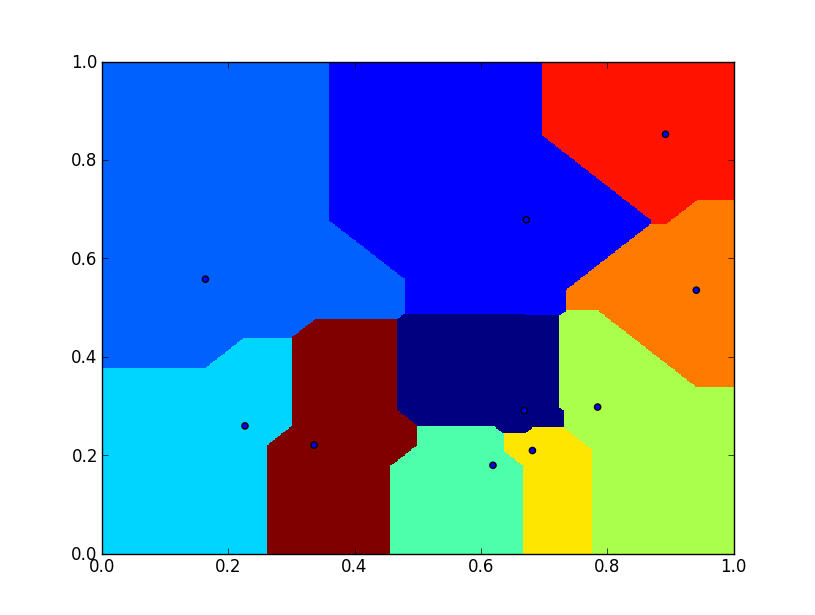
\includegraphics[width=\textwidth]{voronoi_1norm.png}
\caption{Voronoi diagram in the 1-norm}
\label{voronoi_1norm}
\end{minipage}
\hspace{0.5cm}
\begin{minipage}[b]{0.45\linewidth}
\centering
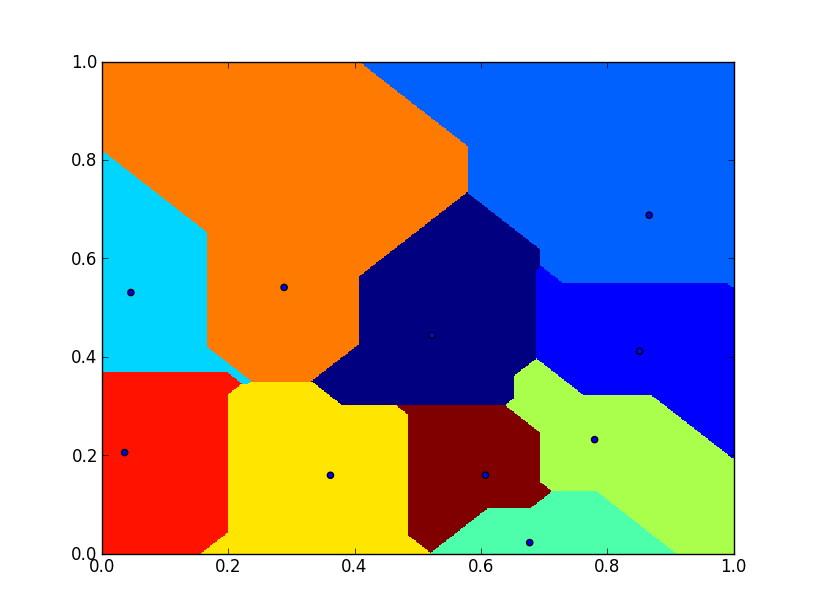
\includegraphics[width=\textwidth]{voronoi_supnorm.png}
\caption{Voronoi diagram in the supremum norm}
\label{voronoi_supnorm}
\end{minipage}
\end{figure}

It is also possible to make voronoi diagrams based off of shapes and lines as well as points. 

There are several data structures used in the field of computational geometry that can store the exact edges of diagrams like this.
We would prefer to not have to worry about sampling the domain in this way.
There are a variety of algorithms that can compute Voronoi diagrams in $\mathcal{O}\left( n \log\left(n\right)\right)$ time (where $n$ is the number of points).
Fortune's algorithm is a linesweep algorithm that can do this.

The Qhull library is commonly used to compute voronoi diagrams, and delaunay triangulations.
SciPy includes a wrapper of the Qhull library in the \li{scipy.spatial} module.
It currently only supports 2 dimensional voronoi diagrams under the Euclidean norm.
It allows you to generate a voronoi diagram from a set of points, add points to a voronoi diagram, find the nearest point to any given point, and plot a voronoi diagram.

A plot similar to the one we just generated can be made using SciPy like this:
\begin{lstlisting}
import numpy as np
from numpy.random import rand
import scipy.spatial as st
from matplotlib import pyplot as plt
G = rand(100,2)
G = st.Voronoi(G)
st.voronoi_plot_2d(G)
plt.xlim((0, 1))
plt.ylim((0, 1))
plt.show()
\end{lstlisting}
Notice how much clearer the plot is and how much faster it is generated.
Try running the last bit of code for 1000 points.
Though this is a little slower than it was for 10 points, this is a graph that would not display well if we had been using the brute force method.

Table \ref{voronoi_attributes} shows the different attributes of the \li{Voronoi} object.
For more details, see \url{http://docs.scipy.org/doc/scipy-dev/reference/spatial.html}
\begin{table}[h!]
\begin{center}
	\begin{tabular}{|l|p{12cm}|}
    \hline

    \li{points} & coordinates of input points (centers of cells)\\

    \li{vertices} & vertices of graph\\

    \li{ridge_points} & indices of the input points between which each ridge on the diagram lies\\

    \li{ridge_vertices} & indices of the vertices at the end of each ridge\\

    \li{regions} & indices of the vertices corresponding to each voronoi cell\\

    \li{point_region} & indices of the regions corresponding to each input point\\

    \hline

    \end{tabular}
\end{center}
\caption{Various summarizing functions}
\label{voronoi_attributes}
\end{table}

Unfortunately, the \li{Voronoi} objects do not allow us to find out, given the coordinates of a new point, which of our original input points lies the closest to it.
To do something like that we would need to use a different algorithm or data structure.
One possible way of solving such a problem is to us a KD tree.
KD trees are discussed in further detail in Volume II.
Scipy includes built in KD trees in both Python and C.
The version in C is generally faster.
You can make a KD tree like this
\begin{lstlisting}
import numpy as np
from numpy.random import rand
import scipy.spatial as st
A = rand(1000,2)
kd = st.cKDTree(A)
\end{lstlisting}
In this case we used the \li{cKDTree} object.
That is a KDTree implemented in C.
\li{KDTree} is a Python-based version that is also included in scipy.
To find the nearest neighbor of a point \li{pt} and how far away it is we can now use the following line of code:
\begin{lstlisting}
kd.query(pt)
\end{lstlisting}
This returns a tuple containing the distance of the given point to the nearest point in \li{A} and the index of that nearest neighbor in \li{A}.
For exmaple, if you put in:
\begin{lstlisting}
kd.query(A[27])
\end{lstlisting}
It will return
\begin{lstlisting}
(0.0,27)
\end{lstlisting}
Since \li{A[27]} would be the nearest point at a distance of \li{0.0}.
\section*{Applications of Voronoi Diagrams}

Though the computation of a Voronoi Diagram does not provide a quick way to run nearest neighbor queries, there are still several applications for Voronoi Diagrams.
The first, and probably most obvious, is the representation of data.
If you want to look for visual patterns in data, a Voronoi Diagram can be very useful.
One historically significant example was the containment of the London Cholera outbreak of 1854.
The English Mathematician John Snow plotted where the cholera outbreaks had all happened and after some consideration, noticed that they were all relatively close to a certain water pump in that portion of the city.
Upon noticing this, he plotted the voronoi cell of that particular water pump and proposed that the cholera outbreak was linked to contaminated water.
He recommended that the pump handle be removed so that people would have to use other pumps in the city.
Once the contaminated pump was shut down, the cholera outbreak was stopped.

Voronoi diagrams can also be used to solve problems involving the points furthest from those already on the graph.
Examples include determining where to drill next when searching for oil, or where to put a new branch of a major company.

The file \li{edge_intersections.py} included with this lab contains a helper function, \li{edge_intersections}, that will be helpful for the rest of the lab.
It takes a Voronoi diagram object as input as well as two tuples (xlims and ylims) representing the limits of a rectangle.
It returns an array containing the intersections of the edges of the voronoi diagram with the boundaries of the rectangular region.
It also returns two lists of pairs of indices.
In the first list of indices, the first index in each pair corresponds to one of the vertices of the Voronoi diagram and the second index corresponds to one of the intersections found by this function.
The second list of indices accounts for the case that no endpoint of an edge intersecting the region lies within the region.
In the second list of indices, both indices of each pair correspond to intersections with the boundaries of the region.

\begin{problem}
\label{FurthestPoints}
Write a function that, given a list of points, \li{pts}, and a rectangular region of the plain and an integer \li{n}, finds the \li{n} points in the region that lie farthest from all the points in \li{pts}.
Do this by creating a list of tuples with the first element as the distance to the nearest neighbor in \li{pts} and the second element of each tuple the canidate point.
You should use a KD tree to compute the distance to the nearest neighbor.
Add to your list of canidate tuples the veritices of the Voronoi diagram, the intersection of the edges given by the helper function, and the corners of the region.
The library \li{heapq} has a nice function \li{nlargest(n,Q)} that will sort your list \li{Q} by the first element in your tuples and return sorted the largest \li{n} elements.
\end{problem}

Another possible application is navigation through a field of obstacles.
This can be done by creating a Voronoi diagram where each obstacle is represented as a point.
This diagram can then be represented as a graph where the vertices of the Voronoi diagram are considered to be the nodes.
Using a shortest path algorithm you can find the shortest path between the two sides that would keep you as far from the obstacles as possible.

\begin{comment}
\begin{problem}
Given a voronoi diagram object, write a function that uses NetworkX to find the shortest path along the edges diagram between any two given vertices.
Have this function take a threshold value to limit which ridges are included.
Do not include a ridge in the adjacency matrix if the distance from the ridge to the center points of the Voronoi cells is less than the threshold.
You can find this distance by measuring the distance between each pair of points referenced in the \li{ridge_points} attribute of the Voronoi object and then dividing by two.
Note: the infinite ridges of the graph have $-1$ listed as one of the indices in the \li{ridge_vertices} attribute.
Make sure you do not include these ridges.

Depending on what is needed from the algorithm, you could modify the weights of the graph to give preference to edges that pass farther from the obstacles.
A fuller solution of this problem would also account for the bounds of the region.
That could be done with the helper function included with this lab.
\end{problem}
\end{comment}

Another possible application of voronoi diagrams is in the estimation of total rainfall, size of ore deposits, or other similar problems.
One simple way to do this is to take a weighted average of all known measurements where each measurement is given the weight corresponding to the size of its voronoi cell.

\begin{comment}
% This problem is cool, but it would probably make the lab too long
% I'll leave it here in case we want to add it later

\begin{problem}
\label{AverageRainfall}
Write a function that, given a square region and measurement values at different nodes, computes the weighted average of the measurements over the region.
Weight each measurement according to the area of the voronoi cell of each node.

Hint: You can find the area of each voroni cell by considering the triangles formed between its vertices and its center point. One way to compute the area of a triangle given the coordinates of its vertices is $A = \sqrt{s\left(s-a\right) \left(s-b\right) \left(s-c\right)}$ where $s = \frac{a+b+c}{2}$ and $a$, $b$, and $c$ are the lengths of the edges of the triangle.
This is known as Herron's Formula.
\end{problem}

\end{comment}

\section*{Delaunay Triangulation}

A concept related to Voronoi diagrams is that of the Delaunay Triangulation.
Delaunay Triangulations also have a wide variety of applications.
One such application is the automatic division of a region into triangles for use in finite element analysis for the numerical solution of partial differential equations.
In general, the delaunay triangulation divides the smallest convex region containing all the given points (the convex hull) into triangles that obey certain rules.

You can make a Delaunay Triangulation from a list of points and plot it like this:
\begin{lstlisting}
A = rand(100, 2)
D = st.Delaunay(A)
plt.triplot(A[:,0] ,A[:,1], D.simplices)
plt.show()
\end{lstlisting}

\begin{problem}
Use a Delaunay triangulation to write a function that breaks up the unit square into right triangles.
Have the only argument to your function be the number of nodes you want along each edge of the square.
Plot your results.
\end{problem}

%other possible applications:
%Use Delaunay Triangulation to tesselate a 3d surface.
%Use tesselation to rerun ore/rainfall problem and compare results.
